% 2009 年湖南卷文科第 15 题：两块斜边长相等的直角三角板拼在一起。
% 来源 PDF：普通高考/2009/2009湖南文.pdf，SHA-256 db41a34b5d57a8db3f2ee49872e3dbc1e290c2e7390fc96cf4e084b5a679e3eb。
% 原页：第 1 页（A3 三栏）第 2 栏下部，书页码 529。
% 重绘依据：按原页拓扑与角度重绘——45° 板为 △ABC（∠A=90°、∠C=45°，故 AC=AB）；
%   30°—60° 板为 △BDE（∠EBD=90°、∠BED=60°、∠BDE=30°），两板斜边 BC 与 ED 相等，
%   故 BE=BC/2、BD=(√3/2)BC；E 在 BC 上，D 在过 B 的 BC 垂线一侧。
%   原页只画 AC、AB、CB、AD、BD、ED 六条线段，A、B 处各有直角标记，
%   C 处有 45° 的角弧、E 处有 60° 的角弧。
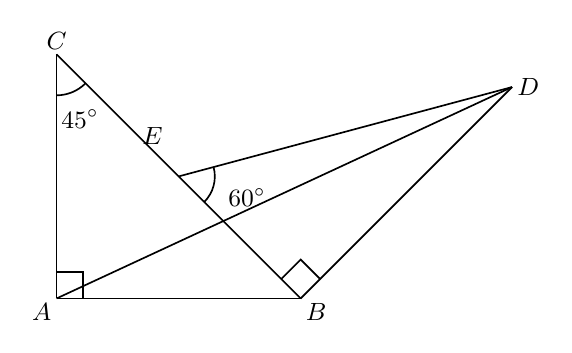
\begin{tikzpicture}[semithick, every node/.style={inner sep=1.6pt, font=\small}]
  % 取 AB=AC=3.1，则 BC=ED=3.1√2≈4.384，BE≈1.55，BD≈2.685
  \coordinate (A) at (0.00,0.00);
  \coordinate (B) at (3.10,0.00);
  \coordinate (C) at (0.00,3.10);
  \coordinate (E) at (1.55,1.55);
  \coordinate (D) at (5.785,2.685);

  % 六条线段
  \draw (A) -- (C);
  \draw (A) -- (B);
  \draw (C) -- (B);
  \draw (A) -- (D);
  \draw (B) -- (D);
  \draw (E) -- (D);

  % A 处直角标记（AC 向上、AB 向右）
  \draw (0.34,0.00) -- (0.34,0.34) -- (0.00,0.34);
  % B 处直角标记（BC 指向左上、BD 指向右上）
  \draw (2.853,0.247) -- (3.100,0.494) -- (3.347,0.247);
  % C 处 45° 角弧（CA 向下、CB 向右下）
  \draw ([shift={(-90:0.52)}]C) arc (-90:-45:0.52);
  % E 处 60° 角弧（EB 向右下、ED 向右上）
  \draw ([shift={(-45:0.46)}]E) arc (-45:15:0.46);

  % 角度标注
  \node at (0.30,2.28) {$45^\circ$};
  \node at (2.42,1.28) {$60^\circ$};

  % 顶点标注
  \node[above] at (C) {$C$};
  \node[below left] at (A) {$A$};
  \node[below right] at (B) {$B$};
  \node[right] at (D) {$D$};
  \node at (1.22,2.06) {$E$};
\end{tikzpicture}
